\documentclass[10pt,pdf,hyperref={unicode}]{beamer}

\usepackage{graphicx}
\graphicspath{{./figs/}}

\mode<presentation> {
	\usetheme{Warsaw}
%	\usetheme{chpc}
	  
	\setbeamercovered{transparent}
  % or whatever (possibly just delete it)
}

\usepackage[english]{babel}
%\usepackage[utf8x]{inputenc}

%\usepackage{amsmath}
\usepackage{bm}
\usepackage{tikz}
\usepackage{pgfplots}

\title[] % (optional, use only with long paper titles)
{A generalized multiscale finite element method for numerical solution of
neutron transport problems in SP$_3$ approximation}

%\subtitle
%{Include Only If Paper Has a Subtitle}

\author[] % (optional, use only with lots of authors)
{\underline{Aleksandr Vasilev \inst{1}} \\
\and Denis Spiridonov \inst{1} \and Aleksandr Avvakumov \inst{2}}
% - Give the names in the same order as the appear in the paper.
% - Use the \inst{?} command only if the authors have different
%   affiliation.

\institute[Universities of Somewhere and Elsewhere] % (optional, but mostly needed)
{
\inst{1} North-Eastern Federal University, Yakutsk, Russia
\\
\vspace{1mm}
\inst{2} National Research Center \textquotedblleft Kurchatov Institute\grqq, Moscow, Russia
}

% - Use the \inst command only if there are several affiliations.
% - Keep it simple, no one is interested in your street address.

\date[July 12-17, 2021] % (optional, should be abbreviation of conference name)
{TEHAC, July 12-17, 2021 Yakutsk}
% - Either use conference name or its abbreviation.
% - Not really informative to the audience, more for people (including
%   yourself) who are reading the slides online

\subject{Theoretical Computer Science}
% This is only inserted into the PDF information catalog. Can be left
% out. 

% ����� � ���������
\graphicspath{{./figs/}}
\newcommand{\grad}{\mathop{\rm grad}\nolimits}
\renewcommand{\div}{\mathop{\rm div}\nolimits}
\newcommand{\const}{\mathop{\rm const}\nolimits}

\begin{document}

\begin{frame}
  \titlepage
\end{frame}

{
  \begin{frame}<beamer>
    \tableofcontents
  \end{frame}
}

\section{Introduction}
\subsection{Introduction}
\begin{frame}{Introduction}
	Real dynamic neutronic calculations require the use of large computational grids during large characteristic times. 
	For these reasons, the reactor calculations can be very expensive.
	\begin{center}
		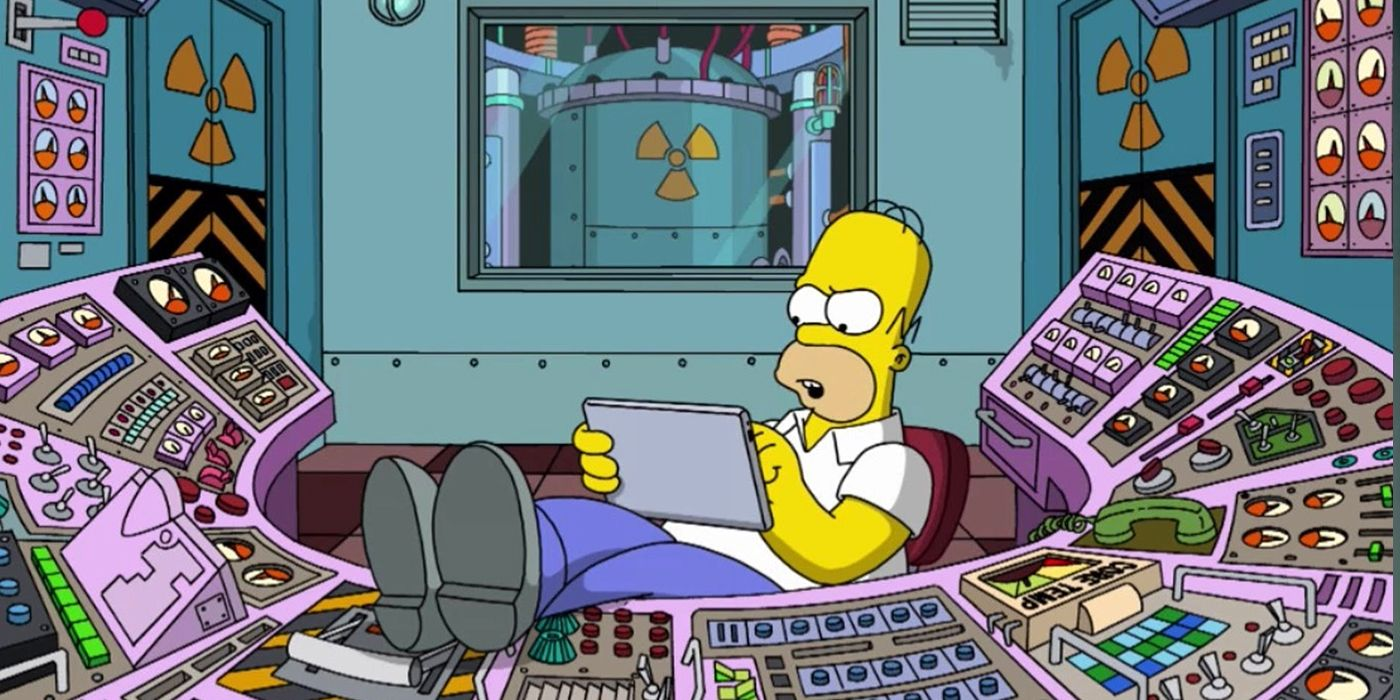
\includegraphics[width=0.7\linewidth] {homer.jpg}	
	\end{center}
	When solving these problems, it is common to use numerical averaging techniques or different multiscale methods that can significantly reduce the number of unknowns, through the construction of coarse-scale model.
\end{frame}

\subsection{Equations}
\begin{frame}{Equations}
	Neutron transport equation: time, energy, spatial and angular variables (7 unknowns)

	\begin{itemize}
		\item Diffusion approximation: one-group, two-group, multi-group
		\item Spherical Harmonics: P$_1$, ..., P$_N$ approximations
		\item Simplified P$_N$: SP$_3$, ..., SP$_N$ approximations
	\end{itemize}
	
	\begin{center}
		
\includegraphics[width=0.7\linewidth] {chernob.jpg}	
	\end{center}
\end{frame}

\section{Problem statement}
\subsection{Diffusion approximation}
\begin{frame}{Problem statement}
	We consider a bounded 2D domain $\Omega$ with a convex boundary $\partial \Omega$. 
	The neutron transport is described by the system of equations
	\[
	\begin{split}
		\frac{1}{v_g} \frac{\partial \phi_{0,g}}{\partial t} - 
		\frac{2}{v_g} \frac{\partial \phi_{2,g}}{\partial t} - 
		& \nabla \cdot D_{0,g} \nabla \phi_{0,g} + 
		  \Sigma_{r,g} \phi_{0,g} -  
		2 \Sigma_{r,g} \phi_{2,g} \\ 
		= & (1 - \beta) \chi_{n,g} S_{n} + S_{s,g} + \chi_{d,g} S_d, \\
		- \frac{2}{v_g} \frac{\partial \phi_{0,g}}{\partial t} + 
		  \frac{9}{v_g} \frac{\partial \phi_{2,g}}{\partial t} - 
		& \nabla \cdot D_{2,g} \nabla \phi_{2,g} + 
		5 \Sigma_{t,g} + 4\Sigma_{r,g}) \phi_{2,g} - 
		2 \Sigma_{r,g} \phi_{0,g} \\
		= & - 2(1 - \beta) \chi_{n,g} S_{n} - 2 S_{s,g} - 2 \chi_{d,g} S_d,
	\end{split}
	\]
	where
	\begin{small}
	\[
		S_{n} = \sum_{g'=1}^{G} \nu \Sigma_{f,g'} \phi_{g'}, \quad
		S_{s,g} = \sum_{g\neq g'=1}^{G} \Sigma_{s,g' \rightarrow g} \phi_{g'}, \quad
		S_{d} = \sum_{m=1}^{M} \lambda_m c_m,
	\]
	\[
		\phi_{0,g} = \phi_g + 2\phi_{2,g}, \quad
		D_{0,g} = \cfrac{1}{3 \Sigma_{tr,g}}, \quad
		D_{2,g} = \cfrac{9}{7 \Sigma_{t,g}}, \quad 
		g = 1,2,\dots,G.
	\]
	\end{small}
\end{frame}

\subsection{Boundary and initial conditons}
\begin{frame}{Boundary and initial conditons}
The density of sources of delayed neutrons
\[
	\frac{\partial c_m}{\partial t} + \lambda_m c_m = \beta_m S_{n}, \quad m = 1,2,\dots,M,
	\quad
	\beta = \sum_{m=1}^{M} \beta_m.
\] 
The Marshak-type boundary conditions ($\partial \Omega$)
\[
\begin{split}
	\begin{bmatrix}
		J_{0,g}(\bm x) \\
		J_{2,g}(\bm x) \\
	\end{bmatrix}
	=
	\begin{bmatrix}
		\phantom{-} \cfrac{1}{2} & - \cfrac{3}{8} \\
	    -\cfrac{3}{8} & \phantom{-} \cfrac{21}{8} \\
	\end{bmatrix}
	\begin{bmatrix}
		\phi_{0,g}(\bm x) \\
		\phi_{2,g}(\bm x) \\
	\end{bmatrix}, \\
	J_{i,g}(\bm x) = - D_{i,g} \nabla \phi_{i,g}(\bm x), \quad i = 0, 2.
\end{split}
\]
The initial conditions
\[
\begin{split}
	\phi_g(\bm x,0) & = \phi_g^0(\bm x), \quad g = 1,2,\dots,G, \\ 
	\quad c_m(\bm x,0) & = c_m^0(\bm x), \quad m = 1,2,\dots,M.
\end{split}
\]

\end{frame}

\subsection{Discretization}
\begin{frame}{Time approximation}
	We assume that at the initial time t = 0, the reactor is in steady-state critical condition.
	\begin{center}
		
\includegraphics[width=0.5\linewidth] {balance.jpg}
	\end{center}
	We discretize the time derivatives of equation using finite-difference scheme. 
	We use a fully implicit scheme with time step $\tau$ for the time approximation.

	For delayed neutron source equation, we use numerical-analytical method
	\[
		c_m^{n+1} = e^{-\lambda_m\tau} c_m^n + 
		\beta_m \int_{t_n}^{t_{n+1}} e^{\lambda_m (t - t^{n+1})} \sum_{g=1}^{G} \nu \Sigma_{fg} \phi_g d t,
		\quad m = 1,2,\dots,M.
	\]
\end{frame}

\begin{frame}{Varitional formulation}
	Let's $H^1(\Omega)$ -- Sobolev space, $q \in H^1$: $q^2$ and $\vert\nabla q\vert^2$ have a finite integral in $\Omega$. 
	Find $\phi^{n+1}_g \in V^G=[H^1(\Omega)]^G$ such that
	\begin{small}
	\[
	\begin{split}
		\int_{\Omega} 
			\left( 
				\frac{\phi^{n+1}_{0,g} - \phi^{n}_{0,g}}{v_g \tau} -
				\frac{2(\phi^{n+1}_{2,g} - \phi^{n}_{2,g})}{v_g \tau} 
			\right) q_g d\bm{x} - & %centering
		\int_{\Omega} D_{0,g} \nabla \phi^{n+1}_{0,g} \nabla q_g d\bm{x} \\
		+ \int_{\partial\Omega} J^{n+1}_{0,g} q_g d\bm{s} +
		\int_{\Omega}
			(
				\Sigma_{r,g} \phi^{n+1}_{0,g} - & %centering
				2\Sigma_{r,g} \phi^{n+1}_{2,g} 
			) q_g d\bm{x} \\
		= \int_{\Omega} 
			(
				(1 - \beta) \chi_{n,g} S^{n+1}_{n} + 
				 S^{n+1}_{s,g} + & %centering
				 \chi_{d,g} S^{n+1}_d 
			) q_g d\bm{x}, \\
		\int_{\Omega} 
			\left( 
				- \frac{2(\phi^{n+1}_{0,g} - \phi^{n}_{0,g})}{v_g \tau} + 
				\frac{9(\phi^{n+1}_{2,g} - \phi^{n}_{2,g})}{v_g \tau} 
			\right) q_g d\bm{x} - & %centering
		\int_{\Omega} D_{2,g} \nabla \phi^{n+1}_{2,g} \nabla  q_g d\bm{x} \\
		+ \int_{\partial\Omega} J^{n+1}_{2,g} q_g d\bm{s} + 
		\int_{\Omega} 
			( 
				(5 \Sigma_{t,g} + 
				4 \Sigma_{r,g}) \phi^{n+1}_{2,g} - & %centering
				2\Sigma_{r,g} \phi^{n+1}_{0,g} 
			) q_g d\bm{x} \\
		= \int_{\Omega}
			( 
				- 2(1 - \beta) \chi_{n,g} S^{n+1}_{n} - 
				2S^{n+1}_{s,g} - & %centering
				2\chi_{d,g} S^{n+1}_d 
			) q_g d\bm{x}.
	\end{split}
	\]
	\end{small}
\end{frame}

\begin{frame}{Discrete problem}
	Further, it's necessary to pass from the continuous variational problem to the discrete problem. 
	We introduce finite-dimensional space of finite elements $V^G_h \subset V^G$ and formulate a discrete variational problem. 
	We use standard linear basis functions as basis functions to solve the problem on the fine grid.
	\vfill
	\begin{center}
		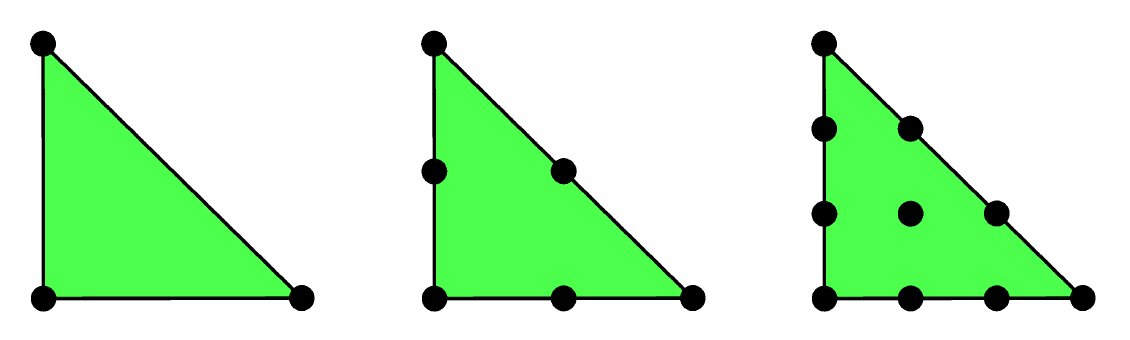
\includegraphics[width=0.4\linewidth] {triangle.png}
	\end{center}
	
	The problem is solving a system of linear algebraic equations
	\[
		A_f \phi = b_f,
	\]
	where operator $A_f$ corresponds to the bilinear form, and the vector $b_f$ corresponds to the linear form.
\end{frame}


\section{Multiscale method}
\subsection{GMsFEM}
\begin{frame}{Multiscale method}
	For the discretization on the coarse grid we use Generalized Multiscale Finite Element Method
(GMsFEM).   
	\begin{center}
		
\includegraphics[width=0.5\linewidth] {mmr.jpeg}
	\end{center}
	GMsFEM involves two basic steps: 
	\begin{enumerate}
	\item The construction of multiscale basis functions that take into
account small scale heterogeneities in local domains;
	\item The construction of the coarse scale approximation.
	\end{enumerate}
\end{frame}

\subsection{Calculation grid}
\begin{frame}{Coarse and fine grids}
	We construct two grids: fine grid ($\mathcal{T}_h$) and coarse grid ($\mathcal{T}_H$). 
	We define local domains $\omega_i$, where $i = 1,...,N_v$ and $N_v$ is the number of coarse grid nodes.
	%We assume that $\mathcal{T}_h$ is a refinement of $\mathcal{T}_H$, where $h$ and $H$ represent the fine and coarse grid sizes, respectively. 
	%We assume that the fine-scale grid $\mathcal{T}_h$ is sufficiently fine to fully resolve the small-scale information of the domain  while $\mathcal{T}_H$ is a coarse grid containing many fine-scale features.

	\begin{figure}[h]
		\centering
		
\includegraphics[width=0.26\linewidth]{coarse_grid.png}
		\hspace{2em}
		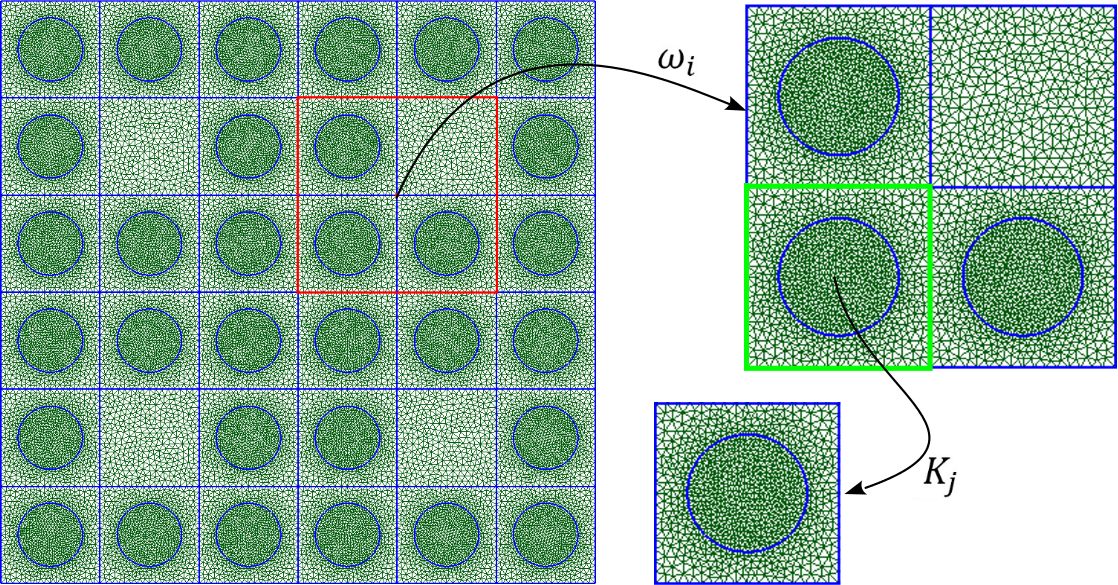
\includegraphics[width=0.5\linewidth]{omega.png} 
		\caption{Coarse grid and local domain $\omega_i$ with $K_j$}
	\end{figure} 

	A local domain $\omega_i$ is obtained by the combining all the coarse cells around one vertex of the coarse grid. 
\end{frame}

\subsection{Spectral problems}
\begin{frame}{Spectral problems}
	For the construction of the multiscale basic functions we solve spectral problems in local
domains. 
	Spectral problems help to identify the most important characteristics of the solution.
	We use following spectral problem in $\omega_i$
	\[
		A \varphi^i = \lambda S \varphi^i,
	\]
	where the elements of the matrices $A= \{ a_{ij} \}$ and $S = \{ s_{ij} \}$ are defined as follow{
	\[
	\begin{split}
		a_{ij} = 
		\int_{\omega_i} D_{0,g} \nabla \phi_{0,g} \nabla q_g d\bm{x} + 
		\int_{\omega_i} (\Sigma_{r,g} \phi_{0,g} - 2\Sigma_{r,g} \phi_{2,g} ) q_g d\bm{x} \\
		-\int_{\omega_i} ((1 - \beta) \chi_{n,g} S_{n} +  S_{s,g} + \chi_{d,g} S_d ) q_g d\bm{x}, \\
		s_{ij} = \int_{\omega _i} D u q d\bm x.
	\end{split}
	\]

	Then, we choose eigenvectors corresponding to dominant $M_{i}$ eigenvalues from \eqref{6} and use them to construct the multiscale basis functions.
\end{frame}

\subsection{Partition of unity functions}
\begin{frame}{Partition of unity functions}
	As  partition of unity functions, we use linear functions in each domain $\omega_i$.
%	Partitions of unity are calculated in the domain $ K_j $ as a linear function from $\Gamma$ to the vertex $ A $, and $ 0 $ is assigned to the entire segment $\Gamma$, and at point $ A $ is assigned the value $1$. 
	Thus, we obtain a linear function from $ 0 $ to $ 1 $ over the entire domain $ K_j $. 
	Domain $K_j$  is one element from a coarse grid. 
	\begin{figure}[h]
		\centering
		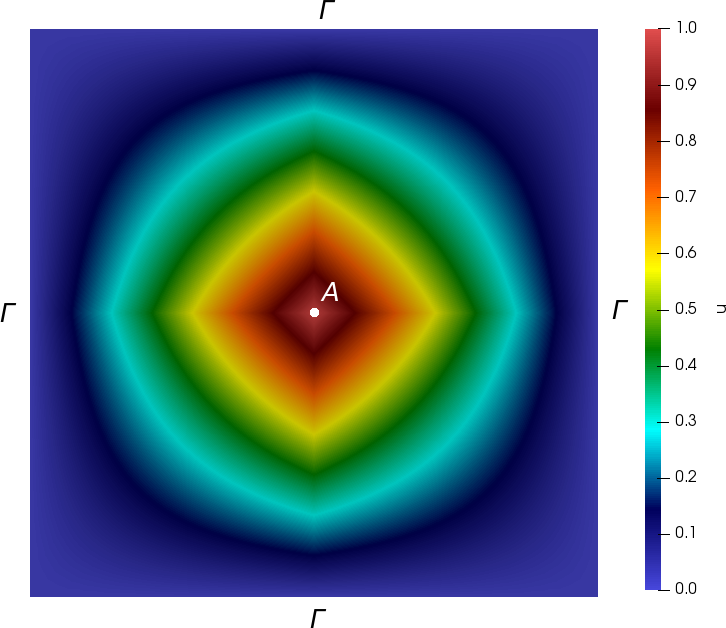
\includegraphics[width=0.3\linewidth]{pofs.png} 
		\hspace{2em}
		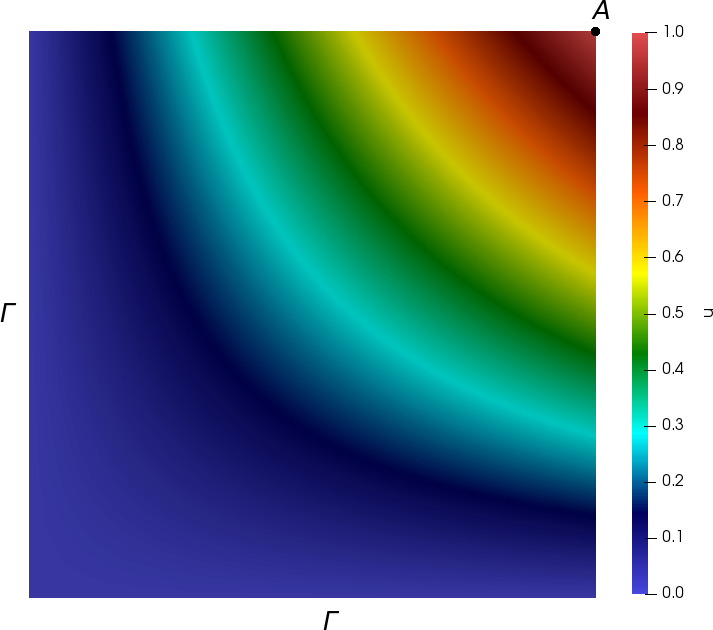
\includegraphics[width=0.3\linewidth]{pouK.png} 
		\caption{Partirion of unity functions on the $\omega_i$ (right) and $K_j$ (left)}
	\end{figure} 
 
	The multiscale space is defined as the span of $y_i = \chi_i \varphi^i_k$, where $\chi_i$ is the usual nodal basis function for the node $i$ (linear partition of unity functions). 
	The number of bases can be different, the accuracy of the solution can be improved when we increase the number of bases.
\end{frame}

\subsection{Coarse-scale approximation}
\begin{frame}{Coarse-scale approximation}
	Next, we create the following  matrix for each $\omega_i$
	\[
		R^i = \left[ y_1, \ldots, y_{M_i-1},  y_{M_i} \right].
	\]
	and define the transition matrix $R$ (transition from a fine grid to a coarse grid) to reduce the dimension of the problem
	\[
		R = [ R^1, R^2, ..., R^{N_v} ].
	\]
	Then using the transition matrix $R$ and fine grid system (\ref{5}), we construct the coarse grid approximation
	\begin{equation}\label{9}
		A_c \phi_c = b_c, \quad 
		A_c = R A_f R^T 
		\quad \text{ and } \quad 
		b_c = R b_f,
	\end{equation}  
	and using the coarse-scale solution $\phi_c$, we can  reconstruct the fine grid solution 
	\[
		\phi_{ms} = R^T \phi_c.
	\]
\end{frame}

\section{Numerical results}
\subsection{Benchmark}
\begin{frame}{Small PWR 2D}
	Let's consider the 2D test problem for small PWR reactor ($\Omega$ --- reactor core area). 
	\begin{figure}[h]
  		\centering
    	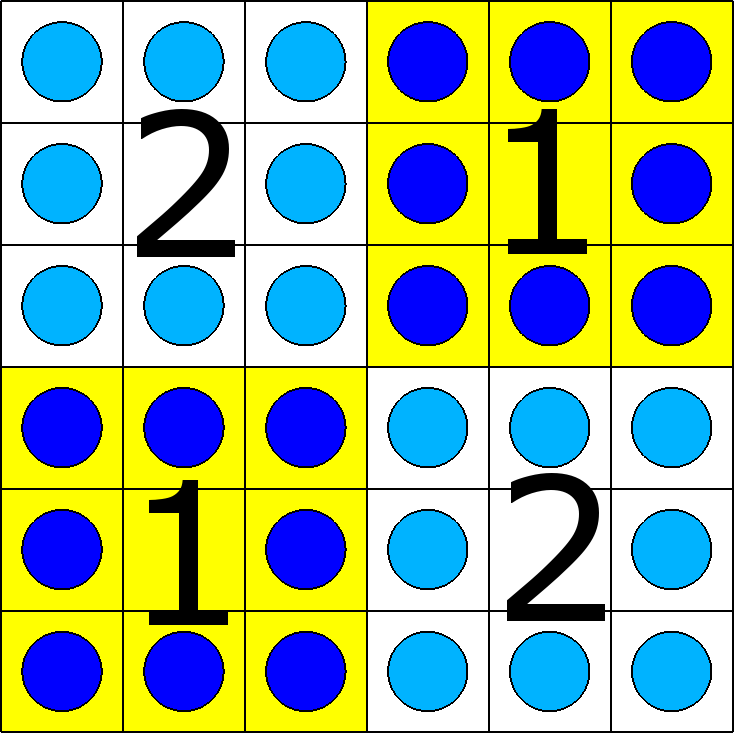
\includegraphics[width=0.3\linewidth] {smallpwr.png}
		\caption{Geometrcial model of the small PWR-2D reactor core}
	\end{figure} 
	The diameter of the fuel rods is 0.82 cm, the cell width is 1.26 cm.
	%Diffusion neutronics constants in the common notations are given in Table \ref{t1}. 
	There are two types of cassettes, with fuel 1\% $UO_2$ and 2\% $UO_2$.
	The reflective boundary conditions (\ref{2}) are used ($\gamma = 0$).
	The following delayed neutrons parameters are used: $\beta = 6.5 \cdot 10^{-3}$, $\lambda = 0.08$ s$^{-1}$ and $v = 5 \cdot 10^5$ cm/s.
\end{frame}

\begin{frame}{Scenario}
We define the next scenario of the process:
\begin{itemize}
\item The $\lambda$-spectral problem is solved and the solution is taken as the initial condition;
\item Calculation for the non-stationary model at the time range from 0 to 0.4 sec;
\item At $t=0.1$ sec and $t=0.3$ sec $\Sigma_a$ for fuel in the zone 1 changes to +2\% and -3\%, respectively (simulation of insertion or withdrawal of control rods).
\end{itemize}
At each time the integrated power is calculated as
\[P(t) = a\int_{\Omega}\Sigma_f \phi d\bm x,\]
where $a$ is the normalization coefficient, which corresponds to a given value of the integrated power.
\end{frame}

\subsection{Software}
\begin{frame}{Software}
\begin{center}
    
\includegraphics[width=0.49\linewidth] {slepc.png}
    \vfill
	
\includegraphics[width=0.49\linewidth] {fenics.png}
\end{center}
\end{frame}

\subsection{Computational results}
\begin{frame}{Fine grid solution}
	The fine grid contains 115891 vertices. 
	The time step for both grids is $\tau = 0.001$.
	As an exact solution, we take the fine-grid solution.
	The initial value of $K_{eff}$ is 1.183280. 

	\begin{figure}[h]
		\centering
		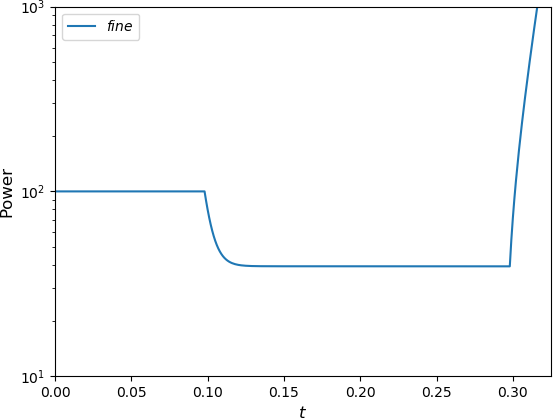
\includegraphics[width=0.55\linewidth]{power_fine.png} 
		\caption{Integral power on the fine grid.}
	\end{figure}
\end{frame}

\begin{frame}{Coarse grid solution}
	The coarse grid contains $49$ vertices.
	When using single basis, the error does not exceed 1\%, and for using 4 or more bases it does not exceed 0.01\%.
	\begin{figure}[h!]
		\centering
		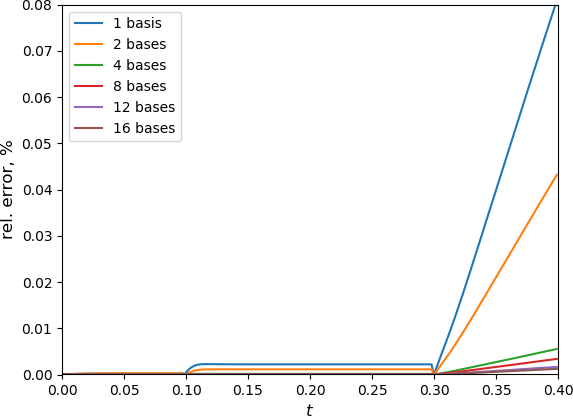
\includegraphics[width=0.55\linewidth]{power.png} 
		\caption{Relative errors ($\%$) of the multiscale solution power.}
	\end{figure}
\end{frame}

\begin{frame}{$L_2$ error}
	We present relative $L_2$ errors of the multiscale solution vs. time for different number of multiscale basis functions.
	The numerical results show good convergence behavior, provided that we take sufficient number of the multiscale basis functions.
\begin{figure}[h]
	\centering
	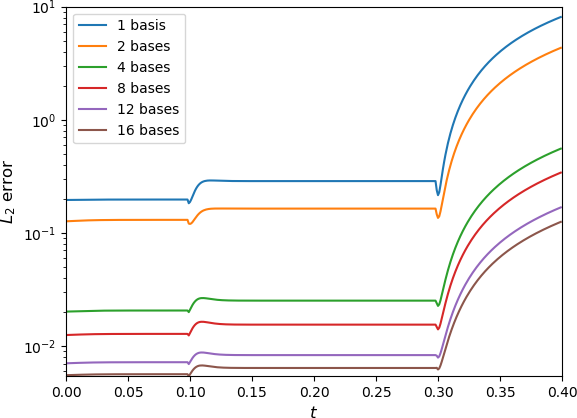
\includegraphics[width=0.55\linewidth]{L2_log.png} 
	\caption{Relative $L_2$ errors ($\%$) of the multiscale solution.}
\end{figure} 
\end{frame}

\begin{frame}{$H_1$ error}
	We present relative $H_1$ errors of the multiscale solution vs. time for different number of multiscale basis functions.
	The numerical results show good convergence behavior, provided that we take sufficient number of the multiscale basis functions.
\begin{figure}[h]
	\centering
	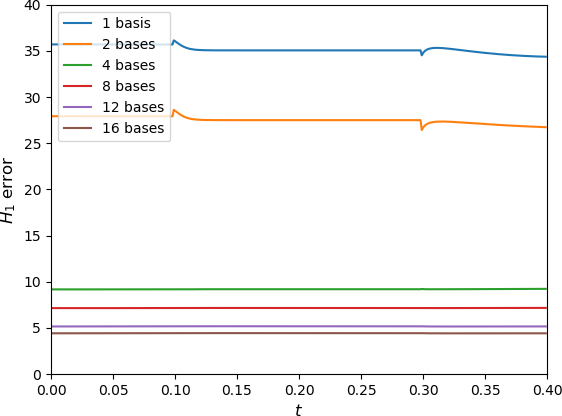
\includegraphics[width=0.55\linewidth]{H1.png} 
	\caption{Relative $H_1$ errors ($\%$) of the multiscale solution.}
\end{figure} 
\end{frame}


\begin{frame}{Errors at final time}
	In Table we present relative $L_2$ and $H_1$ errors at final time for different number of the multiscale basis functions.
	For example, when we use 8 spectral basis functions, we obtain $0.34\%$ for $L_2$ error and $7.18\%$ for $H_1$ error. 
	Our calculations show that it is necessary to use 4 or more basis functions. 
	\begin{table}[h]
		\caption{Relative $L_2$ and $H_1$ errors ($\%$) of the solution at final time.}
		\begin{center}
		\begin{tabular}{|c|c|r|r|r|}
			\hline
			Number of bases & Number of DOF & $L_2$ error & $H_1$ error & Calc time\\
			\hline
			1 & 49 & 8.09 & 34.36 & 0.015 \\
			2 & 98 & 4.32 & 26.73 & 0.018 \\
			4 & 196 & 0.56 & 9.24 & 0.026 \\
			8 & 392 & 0.34 & 7.18 & 0.056 \\
			12 & 588 & 0.17 & 5.17 & 0.102 \\
			16 & 784 & 0.13 & 4.43 & 0.239 \\
			fine & 115891 & -- & -- & 6.816 \\
			\hline
		\end{tabular}
		\end{center}
	\end{table}
\end{frame}

\begin{frame}{Bases}
	We present first four (of 16) multiscale basis functions in local domain $\omega_i$.
	\begin{figure}[h]
		\centering
		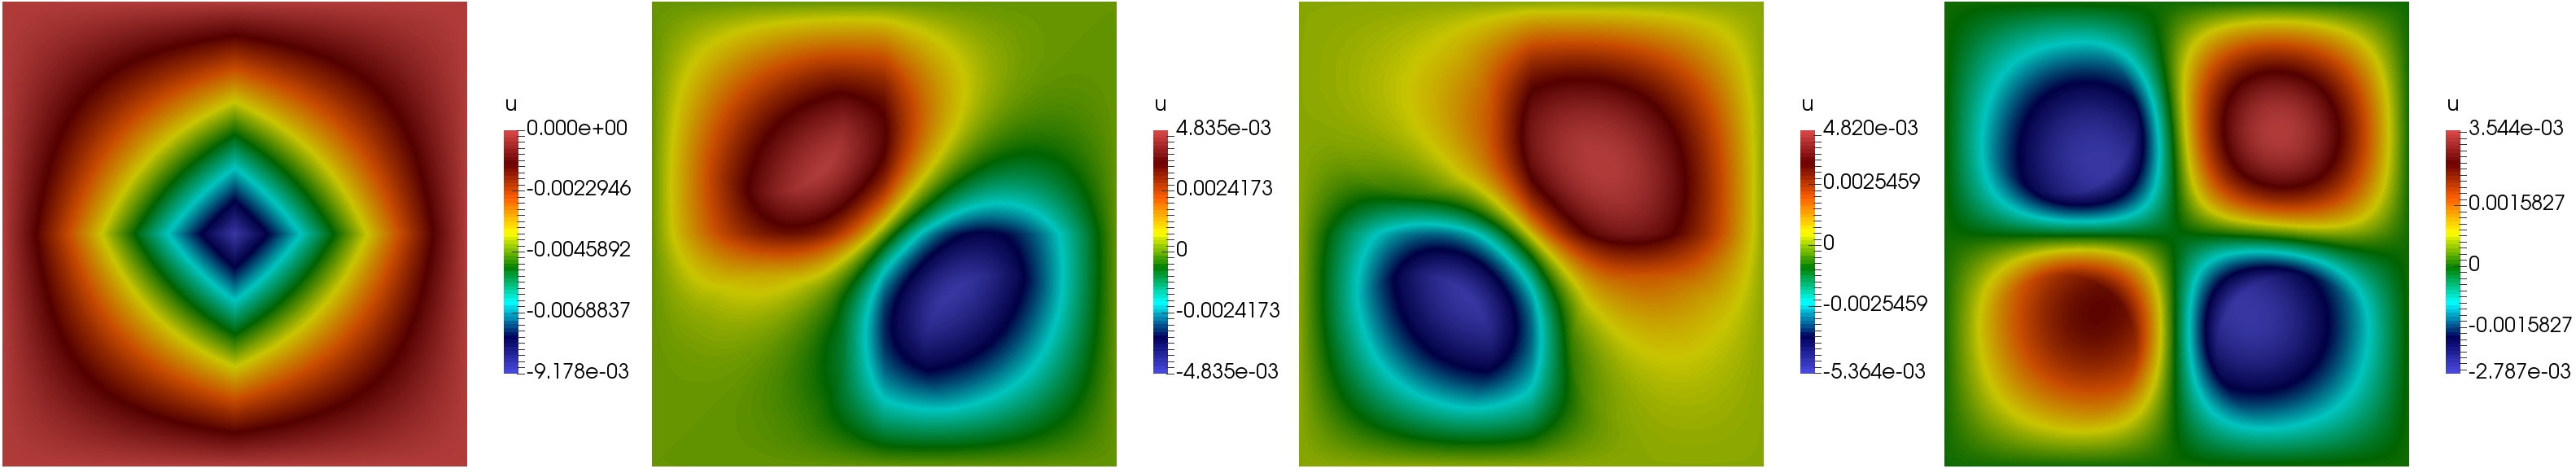
\includegraphics[width=1\linewidth]{basis.png} 
		\caption{The first four multiscale basis functions.}
	\end{figure} 
\end{frame}

\begin{frame}{Neutron flux}
	The fine-grid solution and the multiscale solution (16 basis functions on each local domain) $\omega_i$ are shown in Figure. 
	Relative errors are 0.13\% for $L_2$ and 4.43\% for $H_1$. 
	\begin{figure}[h!]
		\centering
		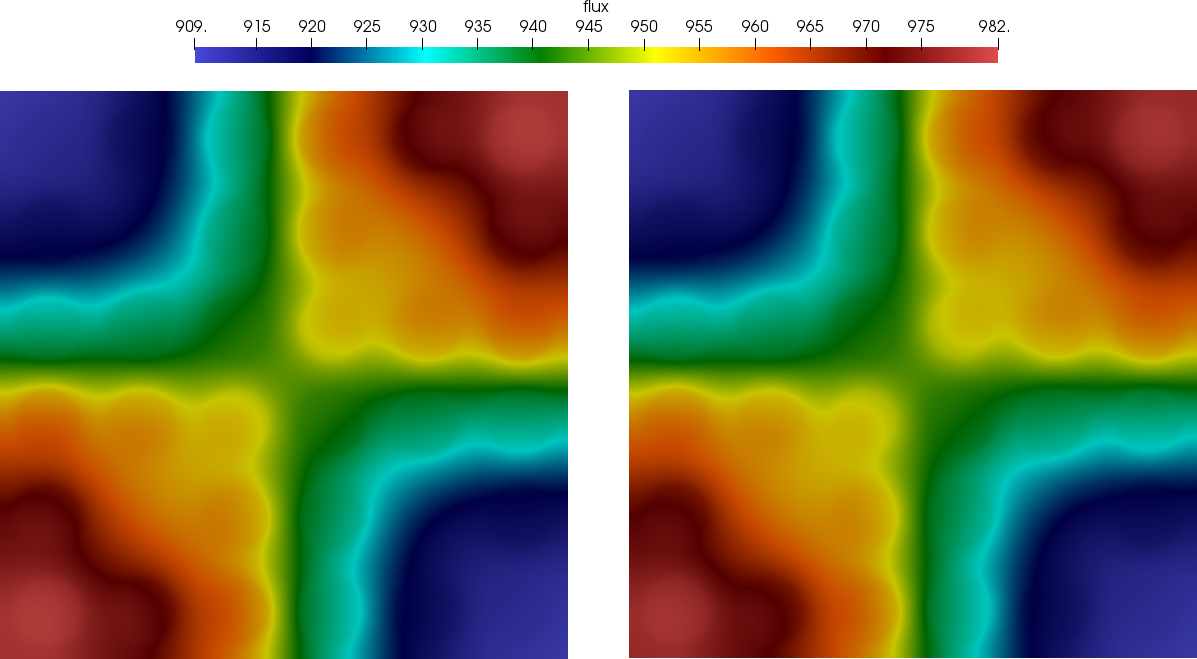
\includegraphics[width=0.75\linewidth]{flux.png} 
		\caption{Fine grid (left) and multiscale solutions (right).}
	\end{figure} 
\end{frame}

\section*{Conclusion}
%\begin{frame}{Acknowledgements}
%This work was supported by the grant of the Russian Science Foundation (\#19-71-00008).
%\end{frame}

\begin{frame}{Conclusion and future work}
	A Generalized Multiscale Finite Element method was developed successfully for modeling neutron transport in one-group diffusion approxmimation.  
	We presented an implementation of GMsFEM. 
	We considered each step of GMsFEM algorithm.
	The results showed that GMsFEM performed with a good accuracy in all considered cases.
\vspace{1em}

	In the current work, we considered the popular and simplest model of neutron transport equation.
	Computational expenses are always an issue even for modern computers.
	In the future, we will consider more complex models of neutron transport, such as $SP_3$ approximation. 
\end{frame}

\begin{frame}
	
\includegraphics[width=1\linewidth]{thanks.jpg} 
\end{frame}

\end{document}
